\section{نتایج}
در این قسمت، چهار روش پیشنهادی روی چهار شاخص پیش‌بینی پیوند که از دستهٔ معیارهای شباهت مبتنی بر همبندی هستند اعمال می‌شوند و مورد ارزیابی قرار می‌گیرند. این شاخص‌ها عبارتند از:

{ \onehalfspacing
\begin{enumerate}
  \item شاخص همسایگان مشترک (\lr{\textit{CN}})
  \item شاخص آدامیک/ادار (\lr{\textit{AA}})
  \item شاخص تخصیص منابع (\lr{\textit{RA}})
  \item شاخص وابستگی ترجیحی (\lr{\textit{PA}})
\end{enumerate}
}

دلیل انتخاب سه شاخص اول، عملکرد بسیار بهتر آن‌ها به نسبت شاخص‌های دیگر (برای مثال شاخص سورنسن یا جاکارد) است. در آزمایشات انجام گرفته، این سه شاخص عملکر عمومی بسیار بهتری از خود نشان می‌دهند و دقت پیش‌بینی آن‌ها زیاد است اما سایر شاخص‌ها دقت مناسبی ندارند. همچنین معیار چهارم یعنی وابستگی ترجیحی نیز به دلیل تفاوت بنیادی آن از نظر ساختاری با سایر شاخص‌ها انتخاب شده است. شاخص‌های دیگر از همه از نظر ساختاری از همسایه‌های مشترک دو گره با ضرایب متفاوت و نرمال‌سازی‌های متفاوت استفاده می‌کنند، اما این شاخص فقط به درجهٔ هر کدام از دو گره توجه می‌کند و به خاطر همین موضوع، پیچیدگی زمانی آن نیز با سایر شاخص‌ها متفاوت است و در حالی که سایر شاخص‌ها پیچیدگی زمانی از مرتبه $O(n^2)$ (یا ضرایب آن) دارند، این شاخص از پیچیدگی زمانی $O(n)$ برخوردار است.

همان‌طور که پیش‌تر گفته شد، برای روش تشخیص انجمن نیز از روش \Infomap استفاده می‌شود. این انتخاب روش بر پایهٔ مطالعهٔ جامع لانچیکینتی و فورتوناتو\LTRfootnote{Fortunato} \cite{lancichinetti2009community} انجام گرفته است. در این مطالعه، این دو محقق نشان دادند که الگوریتم \Infomap به طور کلی روی شبکه‌های \lr{LFR} بهترین عملکرد را دارد و در کل نیز یکی از بهترین روش‌های تشخیص انجمن به شمار می‌رود.

پیش‌تر اشاره شد که برای انجام آزمایشات، از روش ارزیابی متقاطع ۱۰-قسمتی استفاده خواهد شد و نتایج گزارش شده، میانگین ۱۰ بار اجرای الگوریتم خواهد بود. البته در بعضی آزمایش‌ها برای بالا بردن تعداد تکرارها، بیش از یک بار (برای مثال ۳ یا ۵ بار) از ارزیابی متقاطع ۱۰-قسمتی استفاده شده‌است.

هدف این پژوهش در بخش‌های گذشته بررسی عملکرد روش‌های پیشنهادی روی پارامترهای شبکه‌های \lr{LFR} عنوان شد. دو پارامتر اصلی که برای ما از اهمیت ویژه برخوردارند و نحوه توزیع پیوندها و وزن آن‌ها را این شبکه‌ها کنترل می‌کنند، دو پارامتر $\mu_t$ و $\mu_w$ هستند. در نتیجه برای بررسی اثر این پارامتر می‌بایست با تغییر این پارامترها، آزمایشات لازم را انجام داده و نتایج آن‌ها با هم مقایسه شوند. برای این کار مقادیر هر یک از این پارامترها را در بازهٔ $[0.1, 0.7]$ با گام $0.1$ تغییر داده و آزمایشات لازم را انجام می‌شوند. این کار باعث می‌شود که یک فضای پارامتر دو بعدی متشکل از $7 \times 7 = 49$ نقطه داشته باشیم. در ادامه، نتایج آزمایش‌ها برای این ۴۹ نقطه در فضای پارامتر دو بعدی بررسی خواهند شد.

ما این فضای پارامتر دو بعدی را به سه منطقه مانند شکل \ref{fig:3area} تقسیم می‌کنیم: ۱) منطقه‌ای که $\mu_t$ از $\mu_w$ کوچکتر است؛ ۲) منطقه‌ای که $\mu_t$ با $\mu_w$ (به صورت تقریبی) برابر است؛ ۳) منطقه‌ای که $\mu_t$ از $\mu_w$ بزرگتر است. با توجه به تعریف $\mu_t$ و $\mu_w$، نسبت
$1-\mu_t$ از یال‌های شبکه درون انجمن‌ها قرار می‌گیرند و به همین ترتیب
$1-\mu_w$ از مجموع وزن یال‌ها درون انجمن‌ها قرار می‌گیرند.
این به این معناست که اگر
$\mu_t<\mu_w$ باشد، یعنی در منطقه ۱، یال‌هایی که بیرون از انجمن‌ها قرار می‌گیرند به طور میانگین وزن بیشتری نسبت به یال‌هایی دارند که درون انجمن‌ها قرار می‌گیرند، چون نسبت تعداد آن‌ها بیشتر است اما نسبت وزن آن‌ها به آن اندازه نیست. به طور مشابه، وقتی
$\mu_t=\mu_w$ باشد، یعنی در منطقه ۲، میانگین وزن یال‌های درون انجمن با یال‌های بیرون انجمن برابر است و وقتی
$\mu_t>\mu_w$ باشد، یعنی در منطقه ۳، میانگین وزن یال‌های درون انجمن بیشتر از میانگین وزن یال‌های بیرون انجمن است.
اهمیت این موضوع در این است که ما می‌خواهیم پیش‌بینی پیوند را به درون انجمن‌ها محدود کنیم و اثر بخش‌های مختلف فضای پارامتری را بر روی این کار بررسی کنیم.


%So we will have a 7 by 7 grid on parameter space to perform test on. We split this 7 by 7 parameter space to three regions as you can see in Fig. \ref{fig:1}: area \textcircled{\scriptsize{1}} where $\mu_t<\mu_w$, area \textcircled{\scriptsize{2}} where $\mu_t=\mu_w$ and area \textcircled{\scriptsize{3}} where $\mu_t>\mu_w$. According to the definition, $1 - \mu_t$ of links lies inside communities and $1 - \mu_w$ of the sum of link weights lies inside communities. This means that if $\mu_t<\mu_w$, the average weight of the intra-community links is more than the average weight of the inter-community links. Likewise, if $\mu_t=\mu_w$, the average weight of intra-community links is the same as the average weight of inter-community links and if the $\mu_t>\mu_w$, the average weight of intra-community links is less than the average weight of inter-community links. This is important because we want to limit our predictions inside communities and we want to study the effect of different values of parameters on link prediction.
\begin{figure}
  \begin{center}
    \begin{tikzpicture}
    \draw[->] (-0.1,0) -- (4.1,0);
    \draw[->] (0,-0.1) -- (0,4.1);
    \draw[dashed] (0,0) -- (4.0, 4.0);
    \draw [<->] (3.5,2.5) arc (0:90:1);
    \node (mut) at (4, -0.2) {$\mu_t$};
    \node (muw) at (-0.3, 4) {$\mu_w$};
    \node[rotate=90] (lt) at (0.3, 3.0) {\small{$\overline{W_i} < \overline{W_o}$}};
    \node[rotate=45] (eq) at (2.0, 2.0) {\small{$\overline{W_i} \approx \overline{W_o}$}};
    \node[rotate=0 ] (gt) at (3.0, 0.3) {\small{$\overline{W_i} > \overline{W_o}$}};
    \node (Wi) at (2, -0.7) {\scriptsize{$\overline{W_i}$: \rl{میانگین وزن یال‌های درون انجمن}}};
    \node (Wo) at (2, -1.0) {\scriptsize{$\overline{W_o}$: \rl{میانگین وزن یال‌های بیرون انجمن}}};
    \coordinate [label=left:\textcircled{\scriptsize{1}}] (A) at (0.5,0.7);
    \coordinate [label=left:\textcircled{\scriptsize{2}}] (B) at (1,0.7);
    \coordinate [label=left:\textcircled{\scriptsize{3}}] (C) at (1,0.2);
    \end{tikzpicture}
    \caption{نحوه توزیع وزن‌ها در محیط پارامتری دو بعدی $\mu_t-\mu_w$}
    \label{fig:3area}
  \end{center}
\end{figure}

برای سایر پارامترهای شبکه، مقادیر مختلفی آزمایش شده‌است. نتایج کلی به دست آمده در این پژوهش، نسبت به سایر پارامترها الگوی یکسانی را از خود نشان می‌دهد و تقریباً ثابت است. برای آزمایش‌های گزارش شده در این پژوهش، از مقادیر موجود در جدول \ref{tab:LFR_params} استفاده شده‌است.
\begin{table}
  \caption{پارامترهای مورد استفاده برای شبکه‌های \lr{LFR} مورد استفاده در آزمایشات}
  \label{tab:LFR_params}

  \begin{center}
    %\begin{tabular}{r @{ = } r}
    \begin{tabular}{| r | c |}
%       \hline
%       پارامتر & مقدار \\
%       \hline
      \hline
      تعداد گره‌ها & 500 \\
      \hline
      میانگین درجهٔ گره‌ها  &  10 \\
      \hline
      بیشینهٔ درجهٔ گره‌ها  &  50 \\
      \hline
      کمینهٔ اندازهٔ انجمن‌ها &   4 \\
      \hline
      بیشینهٔ اندازهٔ انجمن‌ها & 100 \\
      \hline
    \end{tabular}
  \end{center}
\end{table}

\subsection{نتایج حاصل از با ارزیابی معیار دقت $n$-بهترین}
در این بخش مطابق معمول آزمایش‌های پیش‌بینی پیوند، مقدار $n$ را برابر با ۱۰۰ در نظر می‌گیریم. به دلیل این که تعداد حالت‌های مختلف که می‌بایست این معیار دقت $n$-بهترین را در آن‌ها گزارش کنیم بسیار زیاد است (چهار شاخص، هر کدام در ترکیب با روی چهار روش پیشنهادی، روی ۴۹ نقطه فضای پارامتری) بخشی از این نتایج را به عنوان نمونه گزارش می‌کنیم. الگوی کلی در نتایج نمونه با الگوی کلی در تمام نتایج یکسان است.

در جدول \ref{tab:aa-muw} نتایج دقت $n$-بهترین برای شاخص \lr{AA} به همراه چهار روش پیشنهادی در حالتی که پارامتر $\mu_t$ ثابت و برابر با $0.3$ است و پارامتر $\mu_w$ بین $0.1$ و $0.7$ تغییر می‌کند، نشان داده شده‌است. در این جدول، اعدادی که پررنگ نشان داده شده‌اند دو روش اولی هستند که نتیجه‌ای بهتر از روش پایه داشته‌اند.
\begin{table}[!htb]
\centering
\caption{نتایج به دست آمده برای معیار \lr{AA} همراه چهار روش پیشنهادی در $\mu_t = 0.3$}
\label{tab:aa-muw}
\begin{LTR}
\begin{tabular}{|c|c||c|c|c|c|}
\cline{2-6}
\multicolumn{1}{c|}{} & $AA$ & $AA + WW$ & $AA + WU$ & $AA + UU$ & $AA + UW$ \\ \hline
$\mu_w = 0.1$ & \lr{0.212(35)} & \lr{\textbf{0.213(35)}} & \lr{\textbf{0.213(35)}} & \lr{0.203(40)} & \lr{0.203(40)} \\ \hline
$\mu_w = 0.2$ & \lr{0.236(44)} & \lr{\textbf{0.240(45)}} & \lr{\textbf{0.240(45)}} & \lr{0.234(41)} & \lr{0.234(41)} \\ \hline
$\mu_w = 0.3$ & \lr{0.189(30)} & \lr{0.210(29)} & \lr{0.210(29)} & \lr{\textbf{0.211(32)}} & \lr{\textbf{0.211(32)}} \\ \hline
$\mu_w = 0.4$ & \lr{0.140(26)} & \lr{0.174(27)} & \lr{0.176(28)} & \lr{\textbf{0.184(32)}} & \lr{\textbf{0.182(31)}} \\ \hline
$\mu_w = 0.5$ & \lr{0.100(23)} & \lr{0.048(26)} & \lr{\textbf{0.183(28)}} & \lr{\textbf{0.192(32)}} & \lr{0.066(32)} \\ \hline
$\mu_w = 0.6$ & \lr{0.091(28)} & \lr{0.007(8)} & \lr{\textbf{0.215(42)}} & \lr{\textbf{0.240(43)}} & \lr{0.015(14)} \\ \hline
$\mu_w = 0.7$ & \lr{0.035(17)} & \lr{0.015(13)} & \lr{\textbf{0.137(31)}} & \lr{\textbf{0.168(37)}} & \lr{0.017(14)} \\ \hline
\end{tabular}
\end{LTR}
\end{table}

جدول \ref{tab:aa-mut} نیز متقابلاً دقت $n$-بهترین را برای روش‌های یاد شده در حالتی نشان می‌دهد که $\mu_t$ متغیر است و $\mu_w$ ثابت در نظر گرفته شده است.
\begin{table}[!hbt]
\centering
\caption{نتایج به دست آمده برای معیار \lr{AA} همراه چهار روش پیشنهادی در $\mu_w = 0.3$}
\label{tab:aa-mut}
\begin{LTR}
\begin{tabular}{|c|c||c|c|c|c|}
\cline{2-6}
\multicolumn{1}{c|}{} & $AA$ & $AA + WW$ & $AA + WU$ & $AA + UU$ & $AA + UW$ \\ \hline
$\mu_t = 0.1$ & \lr{0.194(39)} & \lr{0.174(55)} & \lr{\textbf{0.233(41)}} & \lr{\textbf{0.240(45)}} & \lr{0.222(37)} \\ \hline
$\mu_t = 0.2$ & \lr{0.305(41)} & \lr{\textbf{0.334(41)}} & \lr{\textbf{0.334(41)}} & \lr{0.323(41)} & \lr{0.323(41)} \\ \hline
$\mu_t = 0.3$ & \lr{0.186(30)} & \lr{\textbf{0.211(31)}} & \lr{\textbf{0.211(31)}} & \lr{0.195(34)} & \lr{0.195(34)} \\ \hline
$\mu_t = 0.4$ & \lr{0.118(24)} & \lr{\textbf{0.137(19)}} & \lr{\textbf{0.137(18)}} & \lr{0.123(26)} & \lr{0.123(26)} \\ \hline
$\mu_t = 0.5$ & \lr{0.078(27)} & \lr{\textbf{0.083(30)}} & \lr{\textbf{0.080(27)}} & \lr{0.065(25)} & \lr{0.073(27)} \\ \hline
$\mu_t = 0.6$ & \lr{0.076(23)} & \lr{\textbf{0.090(21)}} & \lr{0.066(27)} & \lr{0.051(18)} & \lr{\textbf{0.086(26)}} \\ \hline
$\mu_t = 0.7$ & \lr{0.031(15)} & \lr{0.030(15)} & \lr{0.022(13)} & \lr{0.015(12)} & \lr{\textbf{0.032(14)}} \\ \hline
\end{tabular}
\end{LTR}
\end{table}

اما برای این که بتوان نتیجه‌گیری بهتری از نتایج داشت نیاز است تا معیارهایی داشته باشیم که بازنمایی بهتری داشته باشند. یکی از چالش‌های معیار دقت $n$-بهترین، تعیین $n$ است که می‌تواند تاثیر گذار باشد. به همین دلایل، استفاده از معیاری مثل معیار دقت در $n$ می‌تواند نتایج را روشن‌تر به ما نشان دهد.

\subsection{نتایج حاصل از ارزیابی با معیار دقت در $n$}
همان‌طور که در بخش \ref{subsec:evalu} عنوان شد، این معیار، دقت را به ازای $n$های مختلف در یک نمودار نشان می‌دهد که کمک می‌کند که بتوان مقایسه‌ای به صورت شهودی بین روش‌ها انجام داد. همانند بخش گذشته، به دلیل این که تعداد این نمودارها زیاد است، مجبوریم به ارائهٔ نمونه‌ای از آن‌ها بسنده کنیم. هر نمودار مقایسهٔ روش پایه (یکی از چهار شاخص شباهت انتخاب شده) با چهار روش پیشنهادی که با همان شاخص ترکیب شده‌اند را در یکی از نقاط فضای پارامتر نشان می‌دهد.
برای نمونه، شکل \ref{fig:RAmut01muw05} منحنی‌های دقت در $n$ روش \lr{RA} را به همراه چهار روش پیشنهادی که روی روش \lr{RA} اعمال شده‌اند، در نقطهٔ $\mu_t=0.1,\mu_w=0.5$ نشان می‌دهد. در این شکل واضح است که در این نقطه از فضای پارامترها، روش‌های \lr{WU} و \lr{UU} بسیار نزدیک به هم هستند و از روش پایهٔ \lr{RA} کارایی بهتری دارند و دقت بیشتری ارائه می‌دهند، اما از سوی دیگر روش‌های \lr{WW} و \lr{UW} دقت روش پایه را کاهش می‌دهند. در ادامه، دلیل این رفتار مورد بررسی قرار خواهد گرفت.
\begin{figure}[!htb]
  \begin{center}
    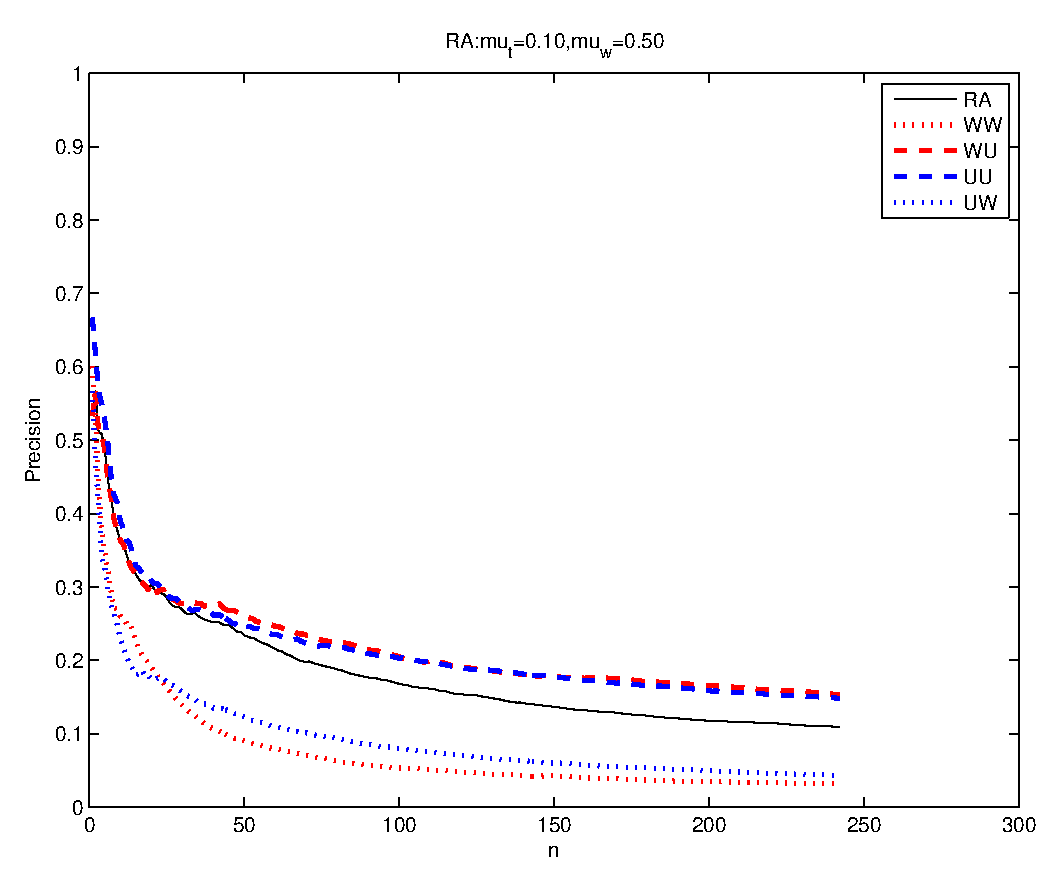
\includegraphics[width=12cm]{RAmut01muw05.eps}
    \caption{معیار دقت در $n$ برای شاخص \lr{RA} و روش‌های پیشنهادی در نقطهٔ $\mu_t=0.1,\mu_w=0.5$}
    \label{fig:RAmut01muw05}
  \end{center}
\end{figure}

شکل‌های \ref{fig:PAmut02muw02} تا \ref{fig:PAmut06muw06} نیز شاخص \lr{PA} را به همراه چهار روش پیشنهادی در چهار نقطه مختلف از فضای پارامتری نشان می‌دهند. همان‌طور که در شکل \ref{fig:PAmut02muw02} مشاهده می‌شود، در نقطهٔ $\mu_t=0.2,\mu_w=0.2$ (که در منطقهٔ ۲ قرار دارد) با استفاده از هر چهار روش پیشنهادی می‌توان به اندازهٔ قابل ملاحظه‌ای دقت پیش‌بینی را بهبود بخشید. در شکل \ref{fig:PAmut02muw06} مشاهده می‌شود که در نقطهٔ $\mu_t=0.2,\mu_w=0.6$ (که در منطقهٔ ۱ قرار دارد) روش‌های UU و WU توانسته‌اند به بهبود دقت پیش‌بینی کمک شایانی بکنند اما دو روش دیگر یعنی WW و UW بهبودی صورت نداده‌اند. در شکل بعد یعنی شکل \ref{fig:PAmut06muw02} در نقطهٔ $\mu_t=0.6,\mu_w=0.2$ (که در منطقهٔ ۳ قرار دارد) برعکس شکل قبل روش‌های WW و UW خوب عمل کرده‌اند اما روش‌های UU و WU نتوانسته‌اند کمک چندانی به پیش‌بینی کنند. در نهایت در شکل \ref{fig:PAmut06muw06}  در نقطهٔ $\mu_t=0.6,\mu_w=0.6$ (که باز هم در منطقهٔ ۲ قرار دارد) هر چهار معیار اندکی توانسته‌اند به بهبود پیش‌بینی کمک کنند.
\begin{figure}[!htb]
  \begin{center}
    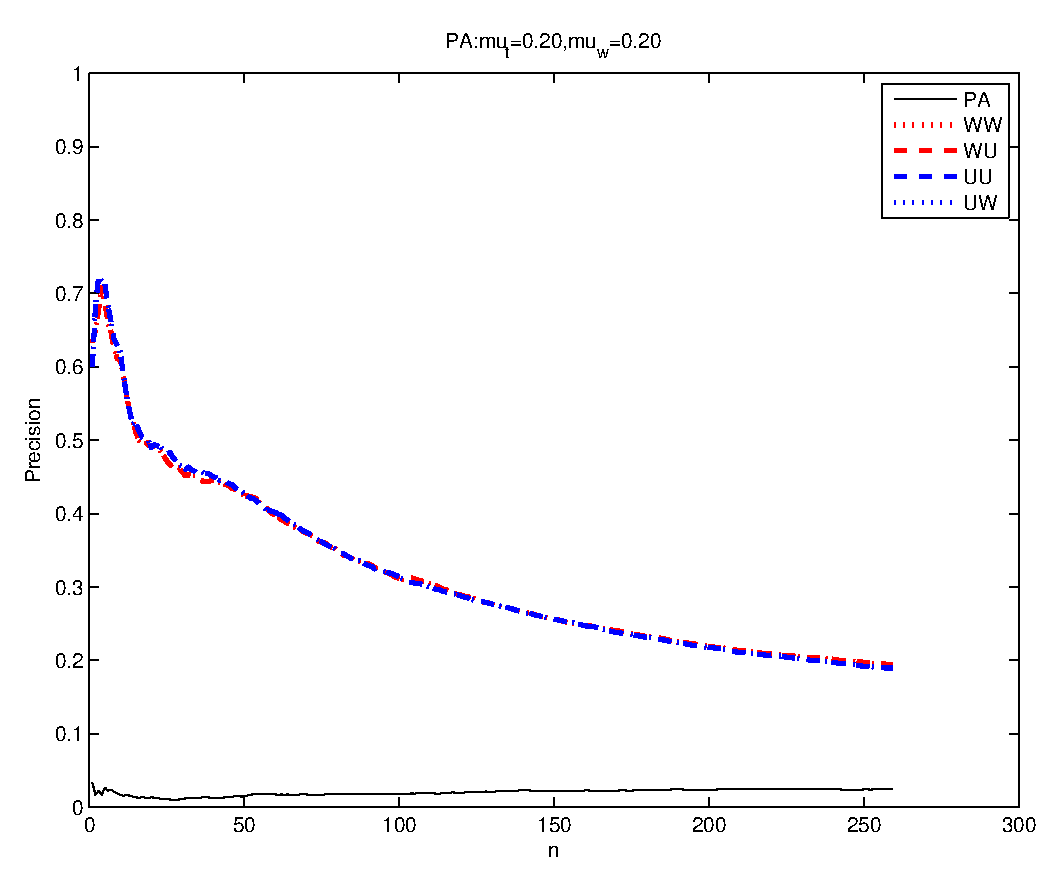
\includegraphics[width=10cm]{PAmut02muw02.eps}
    \caption{معیار دقت در $n$ برای شاخص \lr{PA} و روش‌های پیشنهادی در نقطهٔ $\mu_t=0.2,\mu_w=0.2$}
    \label{fig:PAmut02muw02}
  \end{center}
\end{figure}
\begin{figure}[!htb]
  \begin{center}
    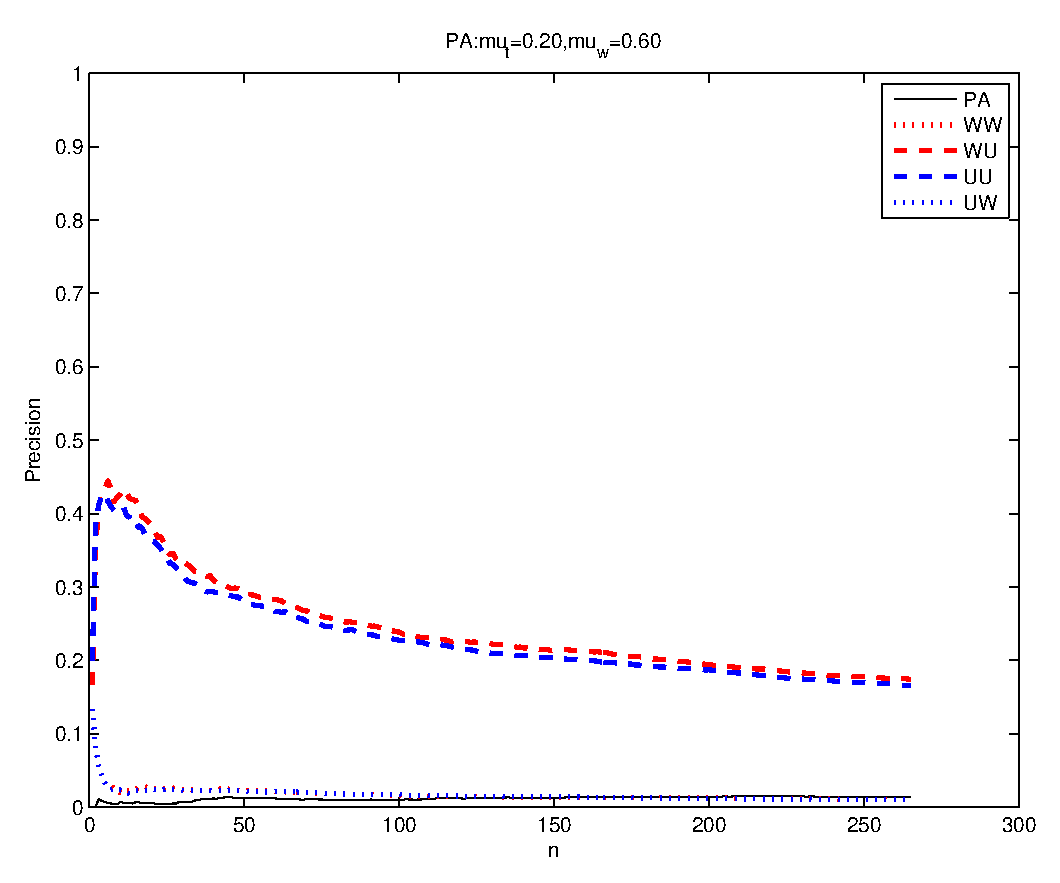
\includegraphics[width=10cm]{PAmut02muw06.eps}
    \caption{معیار دقت در $n$ برای شاخص \lr{PA} و روش‌های پیشنهادی در نقطهٔ $\mu_t=0.2,\mu_w=0.6$}
    \label{fig:PAmut02muw06}
  \end{center}
\end{figure}
\begin{figure}[!htb]
  \begin{center}
    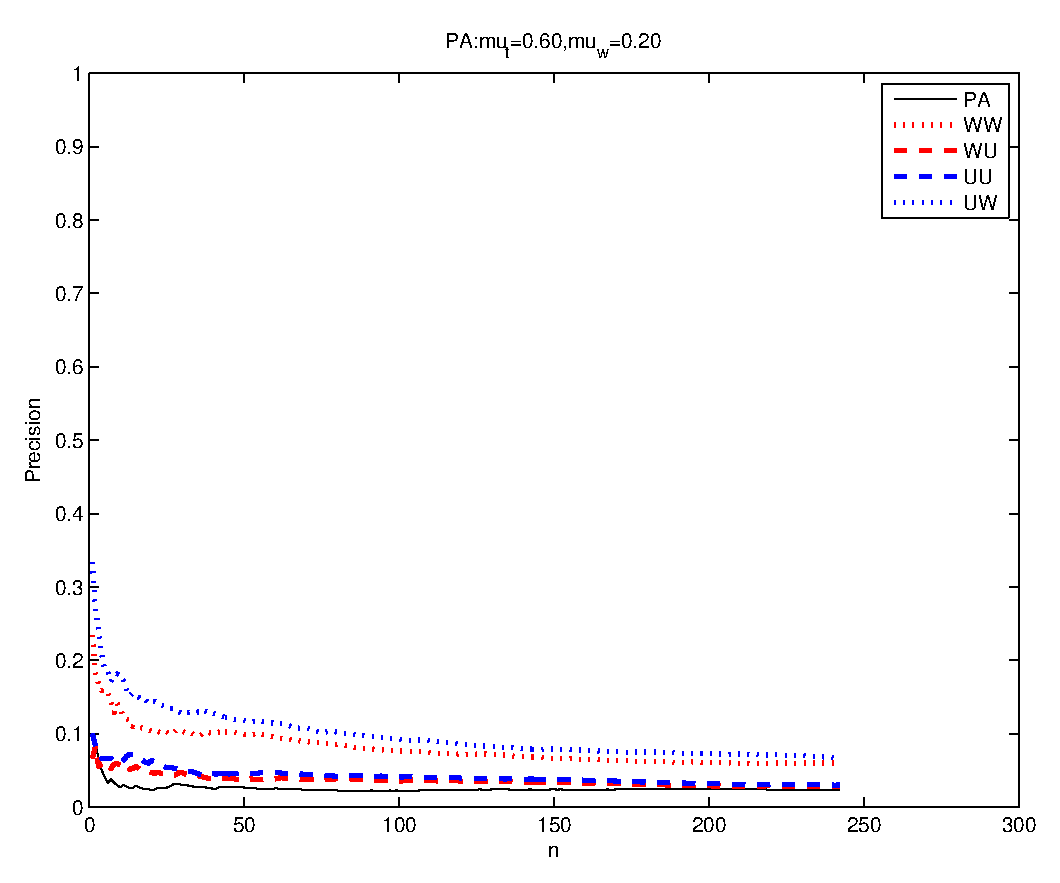
\includegraphics[width=10cm]{PAmut06muw02.eps}
    \caption{معیار دقت در $n$ برای شاخص \lr{PA} و روش‌های پیشنهادی در نقطهٔ $\mu_t=0.6,\mu_w=0.2$}
    \label{fig:PAmut06muw02}
  \end{center}
\end{figure}
\begin{figure}[!htb]
  \begin{center}
    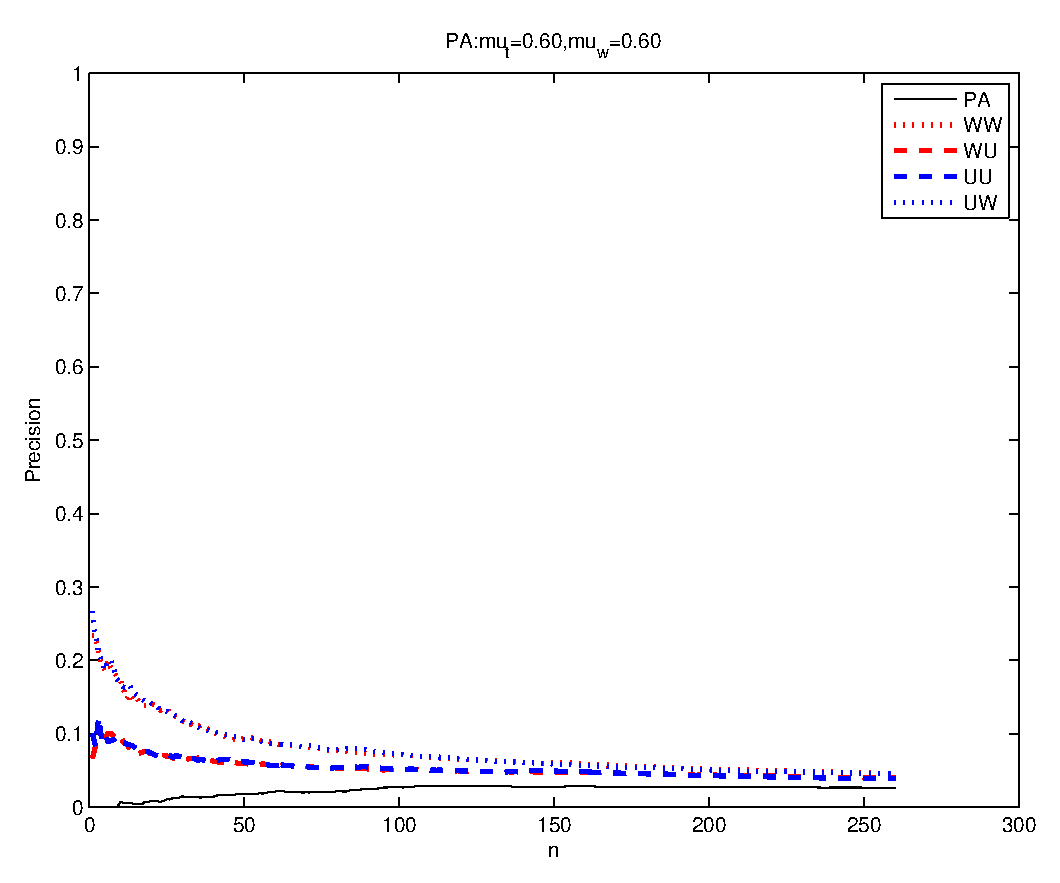
\includegraphics[width=10cm]{PAmut06muw06.eps}
    \caption{معیار دقت در $n$ برای شاخص \lr{PA} و روش‌های پیشنهادی در نقطهٔ $\mu_t=0.6,\mu_w=0.6$}
    \label{fig:PAmut06muw06}
  \end{center}
\end{figure}

اما برای مشاهده تمام این نقاط با هم در یک نمودار واحد می‌بایست روش دیگری را به کار گیریم. در بخش بعد روشی برای این کار معرفی می‌کنیم.

\subsection{نتایج حاصل از ارزیابی با معیار دقت میانگین}
همان‌طور که در بخش‌های قبل اشاره کردیم، هر کدام از منحنی‌های نمودارهای دقت در $n$ را می‌توان با استفاده از رابطهٔ \ref{eq:avgprecision} به یک عدد تبدیل کرد که دقت متوسط نام دارد. از این معیار برای مشاهدهٔ کارایی روش‌ها در نقاط مختلف فضای پارامتری در کنار هم استفاده می‌کنیم. برای این کار، هر کدام از منحنی‌هایی که در نمودارهای دقت در $n$ وجود دارند، به یک عدد تبدیل می‌کنیم، سپس نسبت و یا اختلاف هر یک از چهار روش پیشنهادی در مقایسه با روش پایه به دست می‌آوریم. در نهایت این نسبت و یا را در نموداری رسم می‌کنیم.

با توجه به این که فضای پارامتر ما دو بعدی است و در نتیجه رسم این مقادیر نیاز به فضای سه‌بعدی دارد (که ارائه آن در گزارش امکان‌پذیر نیست)، فضای پارامتر دو بعدی را با استفاده از تبدیل $\mu_t - \mu_w$ به فضای یک بعدی تبدیل می‌کنیم. در نتیجه می‌توان مقادیر به دست آمده را در یک نمودار دو بعدی نشان داد که محور افقی $\mu_t - \mu_w$ و محور عمودی نسبت یا اختلاف را نشان می‌دهد. با استفاده از این تبدیل، می‌توان اثر سه منطقهٔ بحث شده را نیز مشاهده کرد به این صورت که سمت چپ نمودار تا مقدار صفر معادل منطقهٔ ۱، وسط نمودار معادل منطقهٔ ۲ و سمت راست نمودار معادل منطقهٔ ۳ خواهد بود.

شکل‌های \ref{fig:scatter_ratio_CN} تا \ref{fig:scatter_ratio_PA} این نمودارها را به ترتیب برای شاخص‌های
\lr{CN}، \lr{AA}، \lr{RA} و \lr{PA}
در حالتی که نسبت دقت پیش‌بینی مورد نظر بوده، نشان می‌دهند. هر کدام از نقاط روی این شکل‌ها نسبت دقت پیش‌بینی هر یک از روش‌های پیشنهادی به دقت پیش‌بینی روش پایه است که بر حسب اختلاف دو پارامتر $\mu_t$ و $\mu_w$ رسم شده‌اند. همان‌طور که در این شکل‌ها مشخص است در منطقهٔ یک که سمت چپ نمودار است، استفاده از روش‌های \lr{WU} و \lr{UU} توانسته دقت پیش‌بینی بهتری از حالت پایه ارائه کند، اما دو روش دیگر یعنی \lr{WW} و \lr{UW} نتوانسته‌اند تاثیر مثبتی روی دقت پیش‌بینی داشته باشند. هر چه از سمت چپ نمودار به سمت راست حرکت کنیم که معادل حرکت از منطقهٔ ۱ به سمت منطقهٔ ۲ و در نهایت منطقهٔ ۳ است، روش‌های \lr{WU} و \lr{UU} افت کارایی زیادی دارند و از طرف دیگر کارایی دو روش دیگر یعنی \lr{WW} و \lr{UW} بهتر می‌شود.

\begin{figure}[!htb]
  \begin{center}
    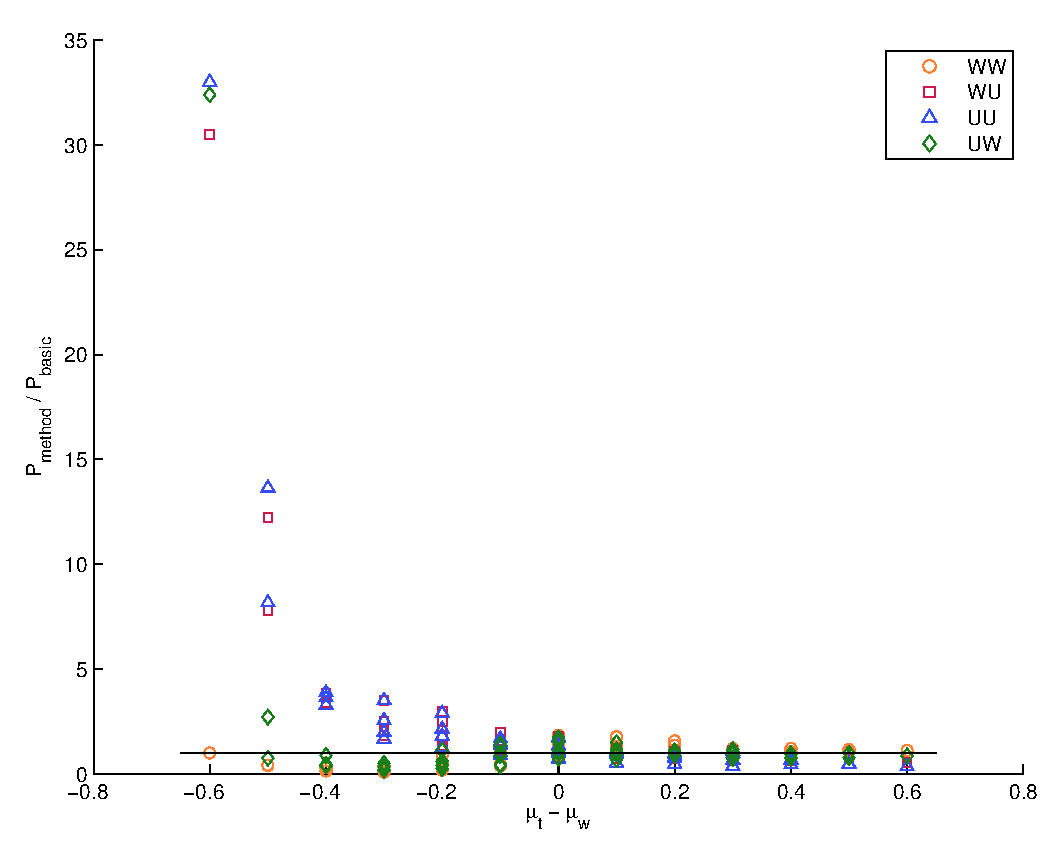
\includegraphics[width=12cm]{scatter_ratio_CN.eps}
    \caption{نسبت بهبود کارایی روش‌های پیشنهادی در معیار \lr{CN}}
    \label{fig:scatter_ratio_CN}
  \end{center}
\end{figure}
\begin{figure}[!htb]
  \begin{center}
    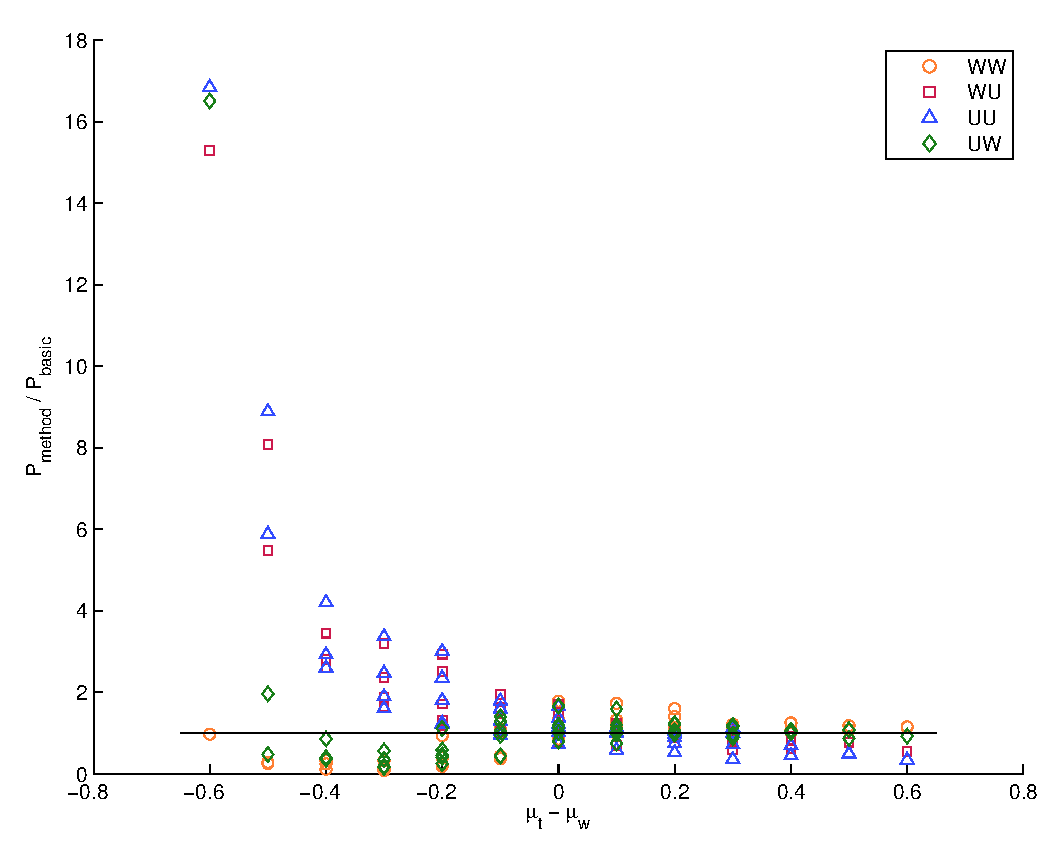
\includegraphics[width=12cm]{scatter_ratio_AA.eps}
    \caption{نسبت بهبود کارایی روش‌های پیشنهادی در معیار \lr{AA}}
    \label{fig:scatter_ratio_AA}
  \end{center}
\end{figure}
\begin{figure}[!htb]
  \begin{center}
    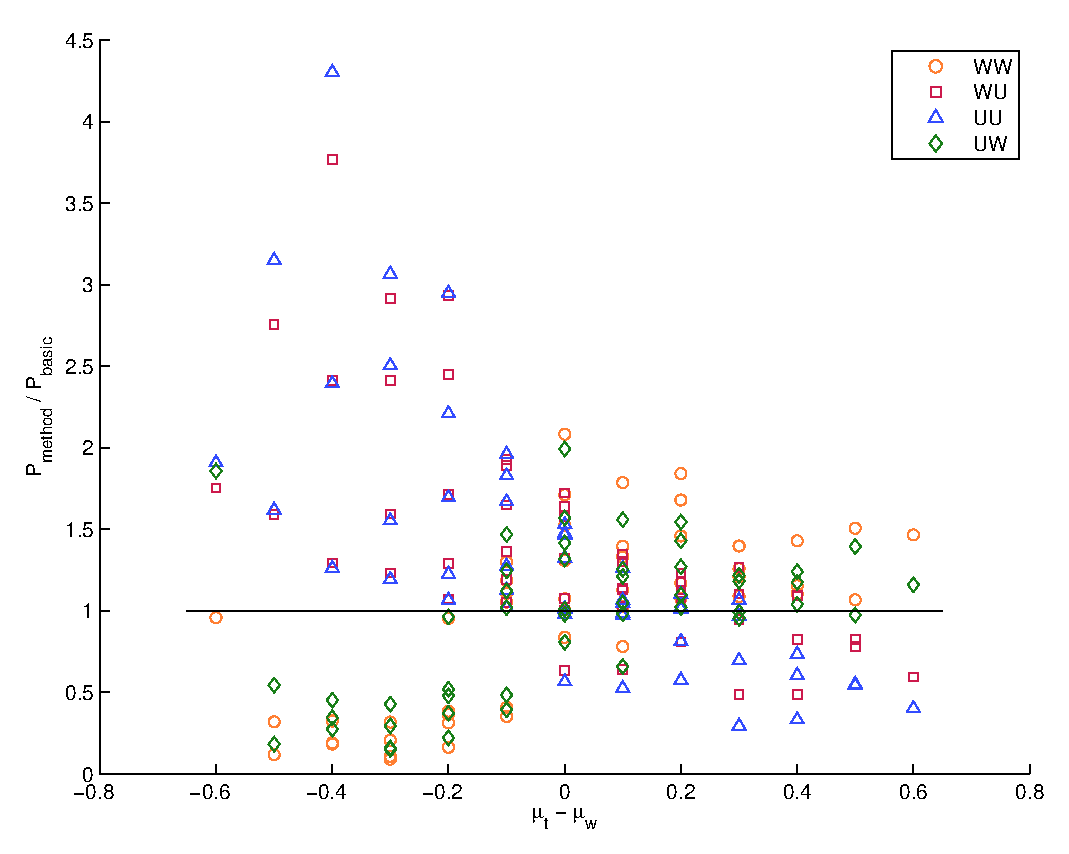
\includegraphics[width=12cm]{scatter_ratio_RA.eps}
    \caption{نسبت بهبود کارایی روش‌های پیشنهادی در معیار \lr{RA}}
    \label{fig:scatter_ratio_RA}
  \end{center}
\end{figure}
\begin{figure}[!htb]
  \begin{center}
    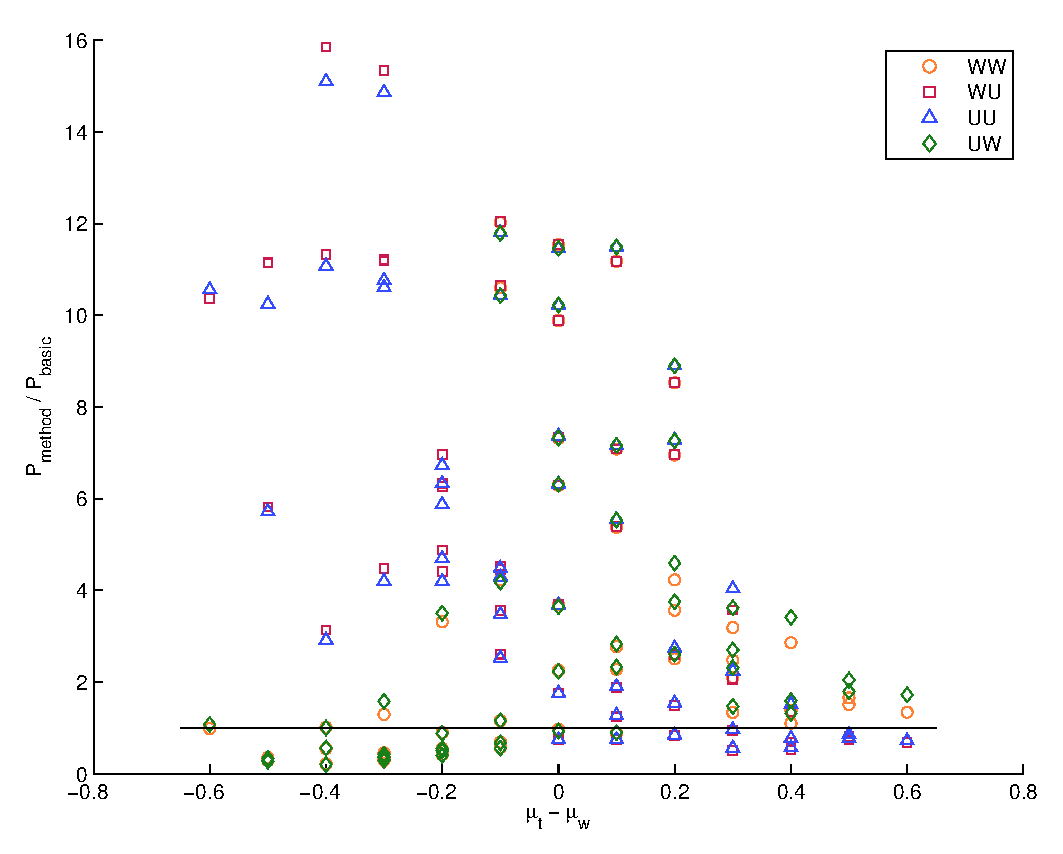
\includegraphics[width=12cm]{scatter_ratio_PA.eps}
    \caption{نسبت بهبود کارایی روش‌های پیشنهادی در معیار \lr{PA}}
    \label{fig:scatter_ratio_PA}
  \end{center}
\end{figure}

شکل‌های \ref{fig:scatter_diff_CN} تا \ref{fig:scatter_diff_PA} نیز مشابه شکل‌های شکل‌های \ref{fig:scatter_ratio_CN} تا \ref{fig:scatter_ratio_PA} هستند با این تفاوت که به جای نسبت، اختلاف دقت پیش‌بینی هر یک از روش‌های پیشنهادی با دقت پیش‌بینی روش پایه را نشان می‌دهند. %این نمودارها نیز تحلیل‌های انجام‌شده را تایید می‌کنند.

\begin{figure}[!htb]
  \begin{center}
    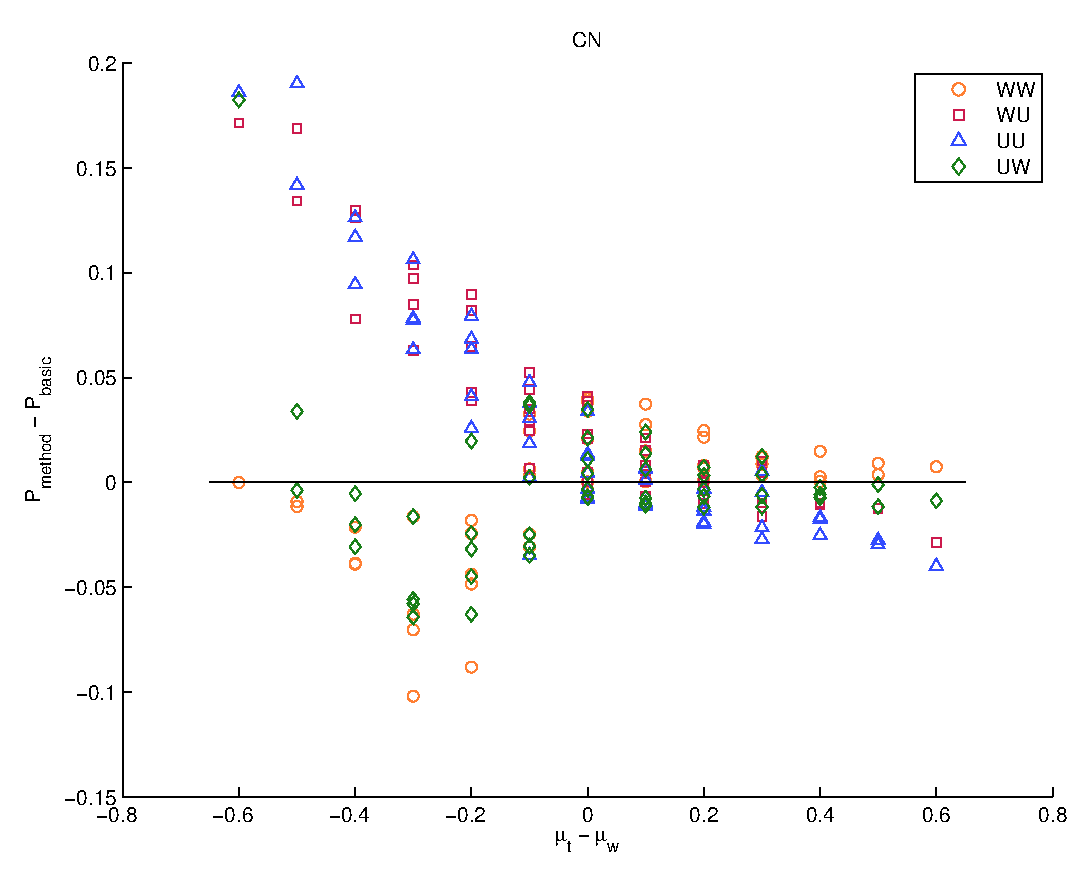
\includegraphics[width=12cm]{scatter_diff_CN.eps}
    \caption{میزان بهبود کارایی روش‌های پیشنهادی در معیار \lr{CN}}
    \label{fig:scatter_diff_CN}
  \end{center}
\end{figure}
\begin{figure}[!htb]
  \begin{center}
    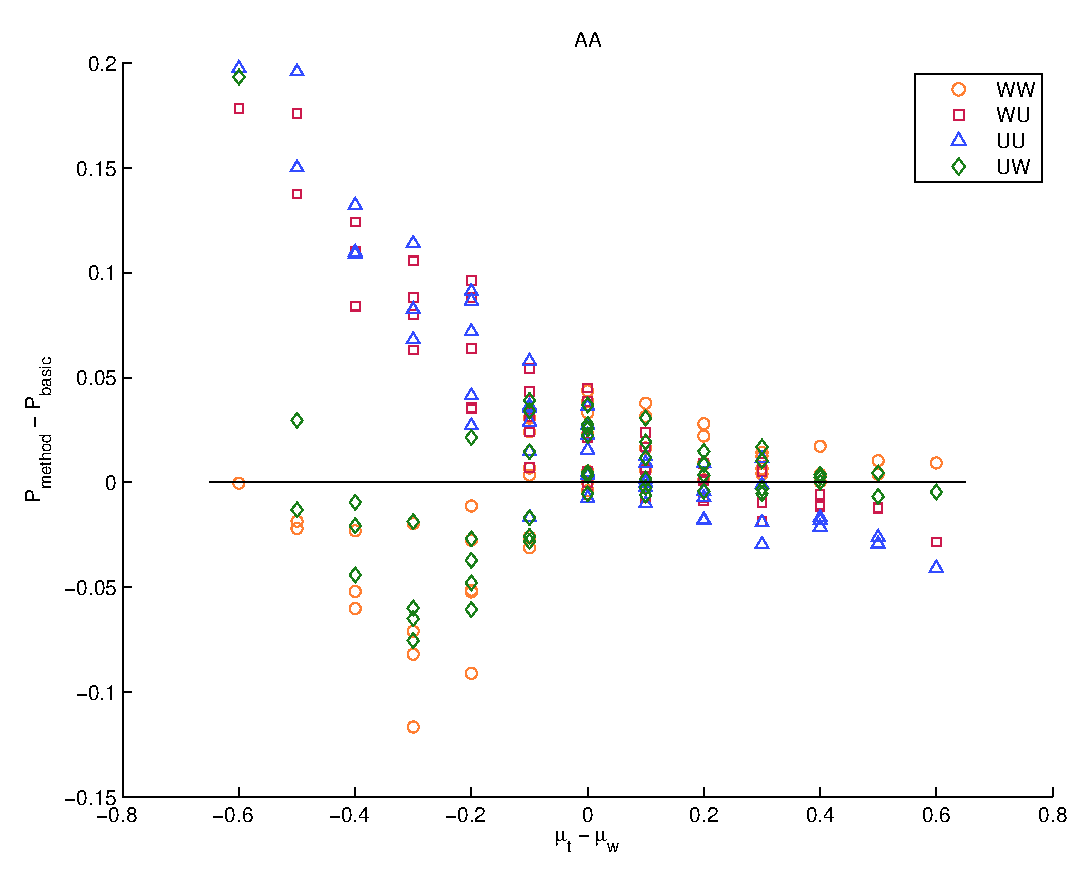
\includegraphics[width=12cm]{scatter_diff_AA.eps}
    \caption{میزان بهبود کارایی روش‌های پیشنهادی در معیار \lr{AA}}
    \label{fig:scatter_diff_AA}
  \end{center}
\end{figure}
\begin{figure}[!htb]
  \begin{center}
    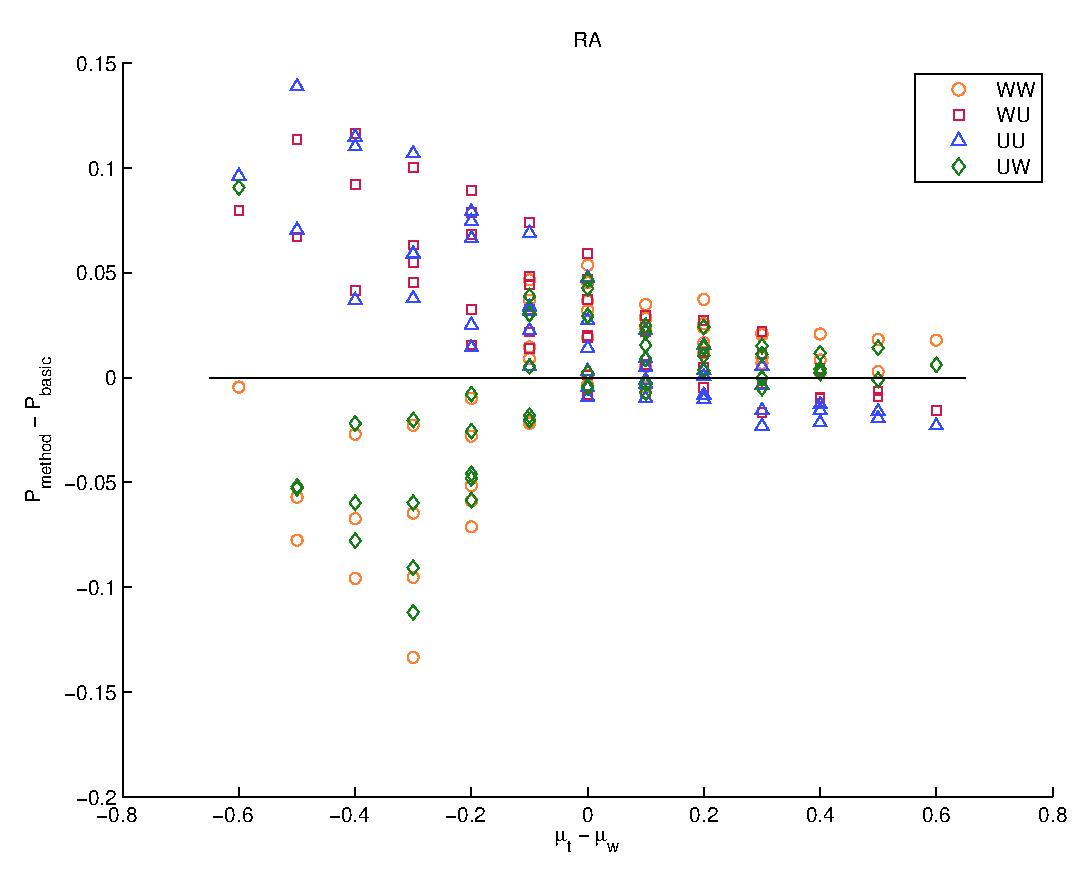
\includegraphics[width=12cm]{scatter_diff_RA.eps}
    \caption{میزان بهبود کارایی روش‌های پیشنهادی در معیار \lr{RA}}
    \label{fig:scatter_diff_RA}
  \end{center}
\end{figure}
\begin{figure}[!htb]
  \begin{center}
    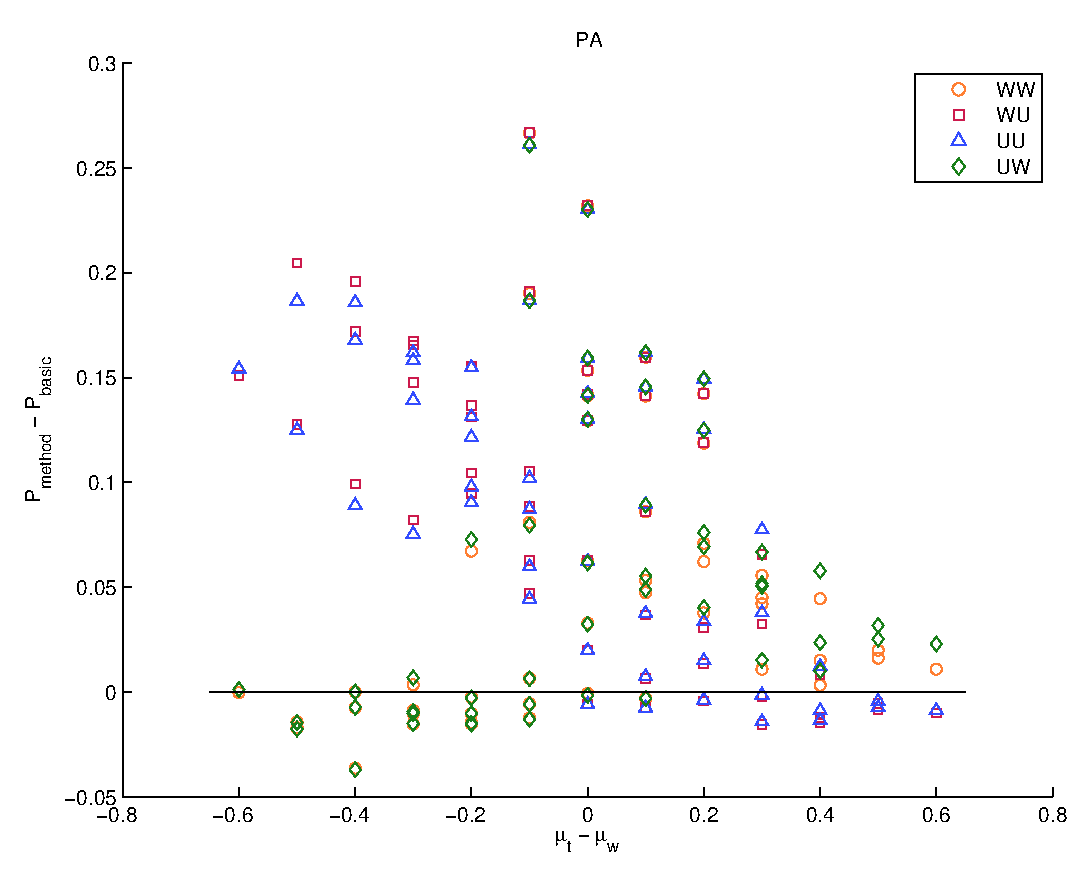
\includegraphics[width=12cm]{scatter_diff_PA.eps}
    \caption{میزان بهبود کارایی روش‌های پیشنهادی در معیار \lr{PA}}
    \label{fig:scatter_diff_PA}
  \end{center}
\end{figure}

%The main reason for this behavior is that in area {{1}} inter-community links are stronger than intra-community links, therefore the weighted community detection algorithm fails to detect true communities properly and this leads to poor prediction precisions. This is because we exclude inter-community potential links from our prediction and with a poor community detection, we might exclude many missing links. But unweighted community detection can detect communities well and therefore, it can help us to improve link prediction performance. In the other hand, in area {{3}}, intra-community links are stronger, therefore although weighted and unweighted community detection are very close, but the weighted version perform better because stronger intra-community links can help the community detection algorithm. As we can see in this figure, in this case, prediction within community helps us to predict more relevant intra-community links and therefore increase precision.

در تحلیل رفتار این روش‌ها در نمودارها، می‌توان گفت که دلیل اصلی این است که در منطقه ۱، یال‌های بین انجمن‌ها قوی‌تر از یال‌های درون انجمن‌هاست. همین قوی‌تر بودن یای‌های بین انجمن‌ها باعث می‌شود که روش‌های تشخیص انجمن وزن‌دار به اشتباه بیافتند و نتواند به نحو مناسبی انجمن‌ها را تشخیص دهند. همین امر باعث می‌شود که دو روش پیشنهادی که از تشخیص انجمن وزن‌دار استفاده می‌کنند، کارایی کمتری داشته باشند و حتا کارایی آن‌ها از روش پایه نیز بدتر شود. اما روش‌های تشخیص انجمن بدون وزن، به دلیل در نظر نگرفتن وزن یال‌ها، خللی در کارشان ایجاد نمی‌شود و می‌توانند به خوبی انجمن‌ها را تشخیص دهند و پیش‌بینی روش‌های پایه را بهبود ببخشند.

اما هر چه از منطقهٔ ۱ فاصله می‌گیریم و به سمت منطقهٔ ۳ می‌رویم، وزن‌یال‌ها درون انجمن‌ها قوی‌تر می‌شوند و در نهایت قوی‌تر از یال‌های بیرون انجمن می‌شوند. این موضوع باعث می‌شود که روش‌های تشخیص انجمنی که از وزن استفاده می‌کنند، انجمن‌های بهتری تشخیص دهند و در نتیجه با این تشخیص انجمن مناسب بتوانند به دقت‌های بهتری برسند. در مقابل نیز روش‌هایی که از اطلاعات وزن استفاده نمی‌کنند با افت کیفیت مواجه می‌شوند چون وزن در این منطقه یک عامل کلیدی است.

\subsection{نتایج حاصل از ارزیابی با معیار \lr{AUC}}
در این بخش نتایج ارزیابی با معیار \lr{AUC} بررسی می‌شود. همانند بخش‌های گذشته به علت حجم بالای خروجی به ارائه نمونه‌ای از آن بسنده می‌شود. سایر نتایج از الگوی مشابهی پیروی می‌کنند. جدول \ref{tab:4-3} مقدار AUC را به ازای $\mu_w = 0.3$ و $\mu_t$ متغیر و جدول \ref{tab:4-4} نیز مقدار AUC را به ازای $\mu_t = 0.3$ و $\mu_w$ متغیر نشان می‌دهد. همان‌طور که از این جداول برمی‌آید، روش‌های پیشنهادی در بیشتر موارد نتوانسته‌اند مقدار AUC را بهبود ببخشند. دلیل این امر این است که روش‌های پیشنهادی، با توجه به ساختارشان نمی‌توانند یال‌هایی که بین انجمن‌ها را تشخیص دهند و همین باعث می‌شود که مقدار AUC افت پیدا کند. البته از طرف دیگر پیش‌بینی‌های اشتباه بین انجمن‌ها نیز رخ نمی‌دهد و این ممکن است باعث بالا رفتن مقدار AUC شود. می‌توان گفت برآیند این دو موضوع در حالت کلی تغییر چندانی در مقدار AUC ایجاد نمی‌کند و همان‌طور که از جدول‌ها مشخص است در اکثر موارد مقادیر AUC به هم نزدیکند. البته باید توجه داشت که معیار AUC معیاریست که کل پیش‌بینی‌ها برای محاسبهٔ آن در نظر گرفته می‌شود. در حالی که معمولاً در کاربردهای مسئلهٔ پیش‌بینی پیوند، کارایی پیش‌بینی در پیش‌بینی‌های ابتدایی مهمتر است تا پیش‌بینی‌های انتهایی. در نتیجه معیارهای دقت اهمیت بیشتری پیدا می‌کنند. %در نهایت با توجه به این که روش‌های پیشنهادی در بیشتر موارد افت چشمگیری نسبت روش پایه ندارند، می‌توان کارایی آن‌ها را با توجه به دقت آن‌ها قابل قبول دانست.

\begin{table}[!htb]
\centering
\caption{نتایج حاصل از ارزیابی معیار \lr{AUC} برای شاخص \lr{CN} به ازای $\mu_w=0.3$}
\label{tab:4-3}
\begin{LTR}
\begin{tabular}{|c|c||c|c|c|c|}
\cline{2-6}
\multicolumn{1}{c|}{} & $CN$ & $CN + WW$ & $CN + WU$ & $CN + UU$ & $CN + UW$ \\ \hline
$\mu_t = 0.1$ & \lr{0.876} & \lr{0.875} & \lr{0.877} & \lr{0.874} & \lr{0.872} \\ \hline
$\mu_t = 0.2$ & \lr{0.776} & \lr{0.778} & \lr{0.774} & \lr{0.773} & \lr{0.775} \\ \hline
$\mu_t = 0.3$ & \lr{0.781} & \lr{0.774} & \lr{0.763} & \lr{0.763} & \lr{0.773} \\ \hline
$\mu_t = 0.4$ & \lr{0.702} & \lr{0.681} & \lr{0.657} & \lr{0.657} & \lr{0.681} \\ \hline
$\mu_t = 0.5$ & \lr{0.679} & \lr{0.645} & \lr{0.601} & \lr{0.601} & \lr{0.645} \\ \hline
$\mu_t = 0.6$ & \lr{0.652} & \lr{0.601} & \lr{0.558} & \lr{0.557} & \lr{0.599} \\ \hline
$\mu_t = 0.7$ & \lr{0.640} & \lr{0.549} & \lr{0.602} & \lr{0.601} & \lr{0.549} \\ \hline
\end{tabular}
\end{LTR}
\end{table}


\begin{table}[!htb]
\centering
\caption{نتایج حاصل از ارزیابی معیار \lr{AUC} برای شاخص \lr{CN} به ازای $\mu_t=0.3$}
\label{tab:4-4}
\begin{LTR}
\begin{tabular}{|c|c||c|c|c|c|}
\cline{2-6}
\multicolumn{1}{c|}{} & $CN$ & $CN + WW$ & $CN + WU$ & $CN + UU$ & $CN + UW$ \\ \hline
$\mu_w = 0.1$ & \lr{0.781} & \lr{0.774} & \lr{0.763} & \lr{0.763} & \lr{0.773} \\ \hline
$\mu_w = 0.2$ & \lr{0.755} & \lr{0.742} & \lr{0.740} & \lr{0.738} & \lr{0.742} \\ \hline
$\mu_w = 0.3$ & \lr{0.754} & \lr{0.728} & \lr{0.738} & \lr{0.737} & \lr{0.726} \\ \hline
$\mu_w = 0.4$ & \lr{0.743} & \lr{0.660} & \lr{0.738} & \lr{0.736} & \lr{0.660} \\ \hline
$\mu_w = 0.5$ & \lr{0.744} & \lr{0.508} & \lr{0.744} & \lr{0.742} & \lr{0.508} \\ \hline
$\mu_w = 0.6$ & \lr{0.753} & \lr{0.505} & \lr{0.759} & \lr{0.757} & \lr{0.505} \\ \hline
$\mu_w = 0.7$ & \lr{0.762} & \lr{0.510} & \lr{0.769} & \lr{0.768} & \lr{0.511} \\ \hline
\end{tabular}
\end{LTR}
\end{table}
